% Rules for the HuroCup Marathon Competition
% Jacky Baltes <jacky@cs.umanitoba.ca> 

\documentclass[12pt]{hurocup}

\begin{document}

\title{\HuroCup: Marathon\\
  Laws of the Game 2008}


\author{Jacky Baltes\\
Autonomous Agents Laboratory\\
University of Manitoba\\
Winnipeg, Manitoba\\
Canada, R3T 2N2\\
Email: jacky@cs.umanitoba.ca\\
WWW: http://www.cs.umanitoba.ca/\~{ }jacky
}

\maketitle

\begin{center}
 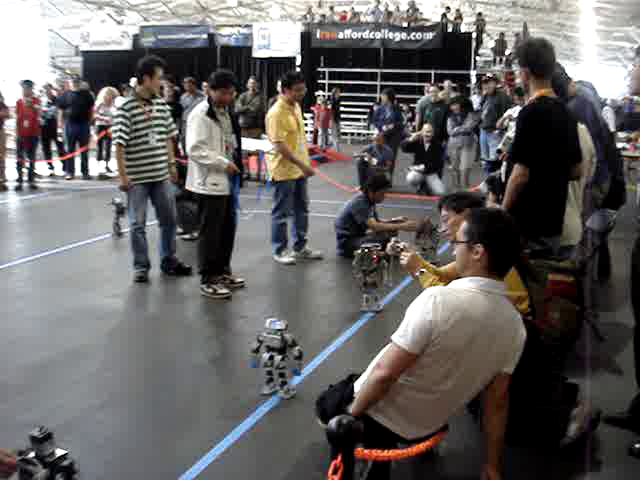
\includegraphics[width=0.7\linewidth]{Figures/marathon-life}
\end{center}

\begin{abstract}
The following rules and regulations govern the Marathon event in
\HuroCup, a robotic game and robotics benchmark problem for humanoid
robots.
%
\end{abstract}

\section*{Latest Version of the Rules for \HuroCup}
\label{sec:updates}

The latest official version of the rules of the game for \HuroCup\ is
always available from the FIRA \HuroCup\ website (http://www.fira.net).

\newpage

\section{Marathon}
\label{sec:marathon} 

Similar to the human marathon run, the \HuroCup\ marathon aims to test
the robustness and endurance of humanoid robots. The task is for the
robot to track a visible line for a distance of 42.195m (1/1000 of a
human marathon distance) as quickly as possible. 

\section{Changes in the Laws of \HuroCup\ Marathon for 2008}

There are no significant changes in the laws of the marathon event
between 2007 and 2008.

\section{Laws of the Game: Marathon}
\label{sec:marathon-laws}

The following laws describe the specifics of the marathon
event. For general specifications relevant to all \HuroCup\ events
(e.g., robot dimensions, playing field and lighting, responsibility of
the referees) please refer to the general \HuroCup\ laws.

\law[MR]{The Field of Play}
\label{mr-field}

\begin{lawlist}[MR]

\item The track for the marathon event is on an even surface.

\item The centre of the track is marked with a 4 - 8cm wide coloured
line, called the centre line.

\item The length of the centre line is 4219.5 cm.

\item The centre line does not include any corners with an
 angle of more than 90 degrees or turns with a turn radius of less
 than 1m.

\item The centre line does not contain any intersections.

\item The minimum distance between points on the centre line that
 belong to different segments is at least 100cm.  See
 Fig.~\ref{fig:marathon-track} for an example.

\begin{figure}
  \begin{center}
    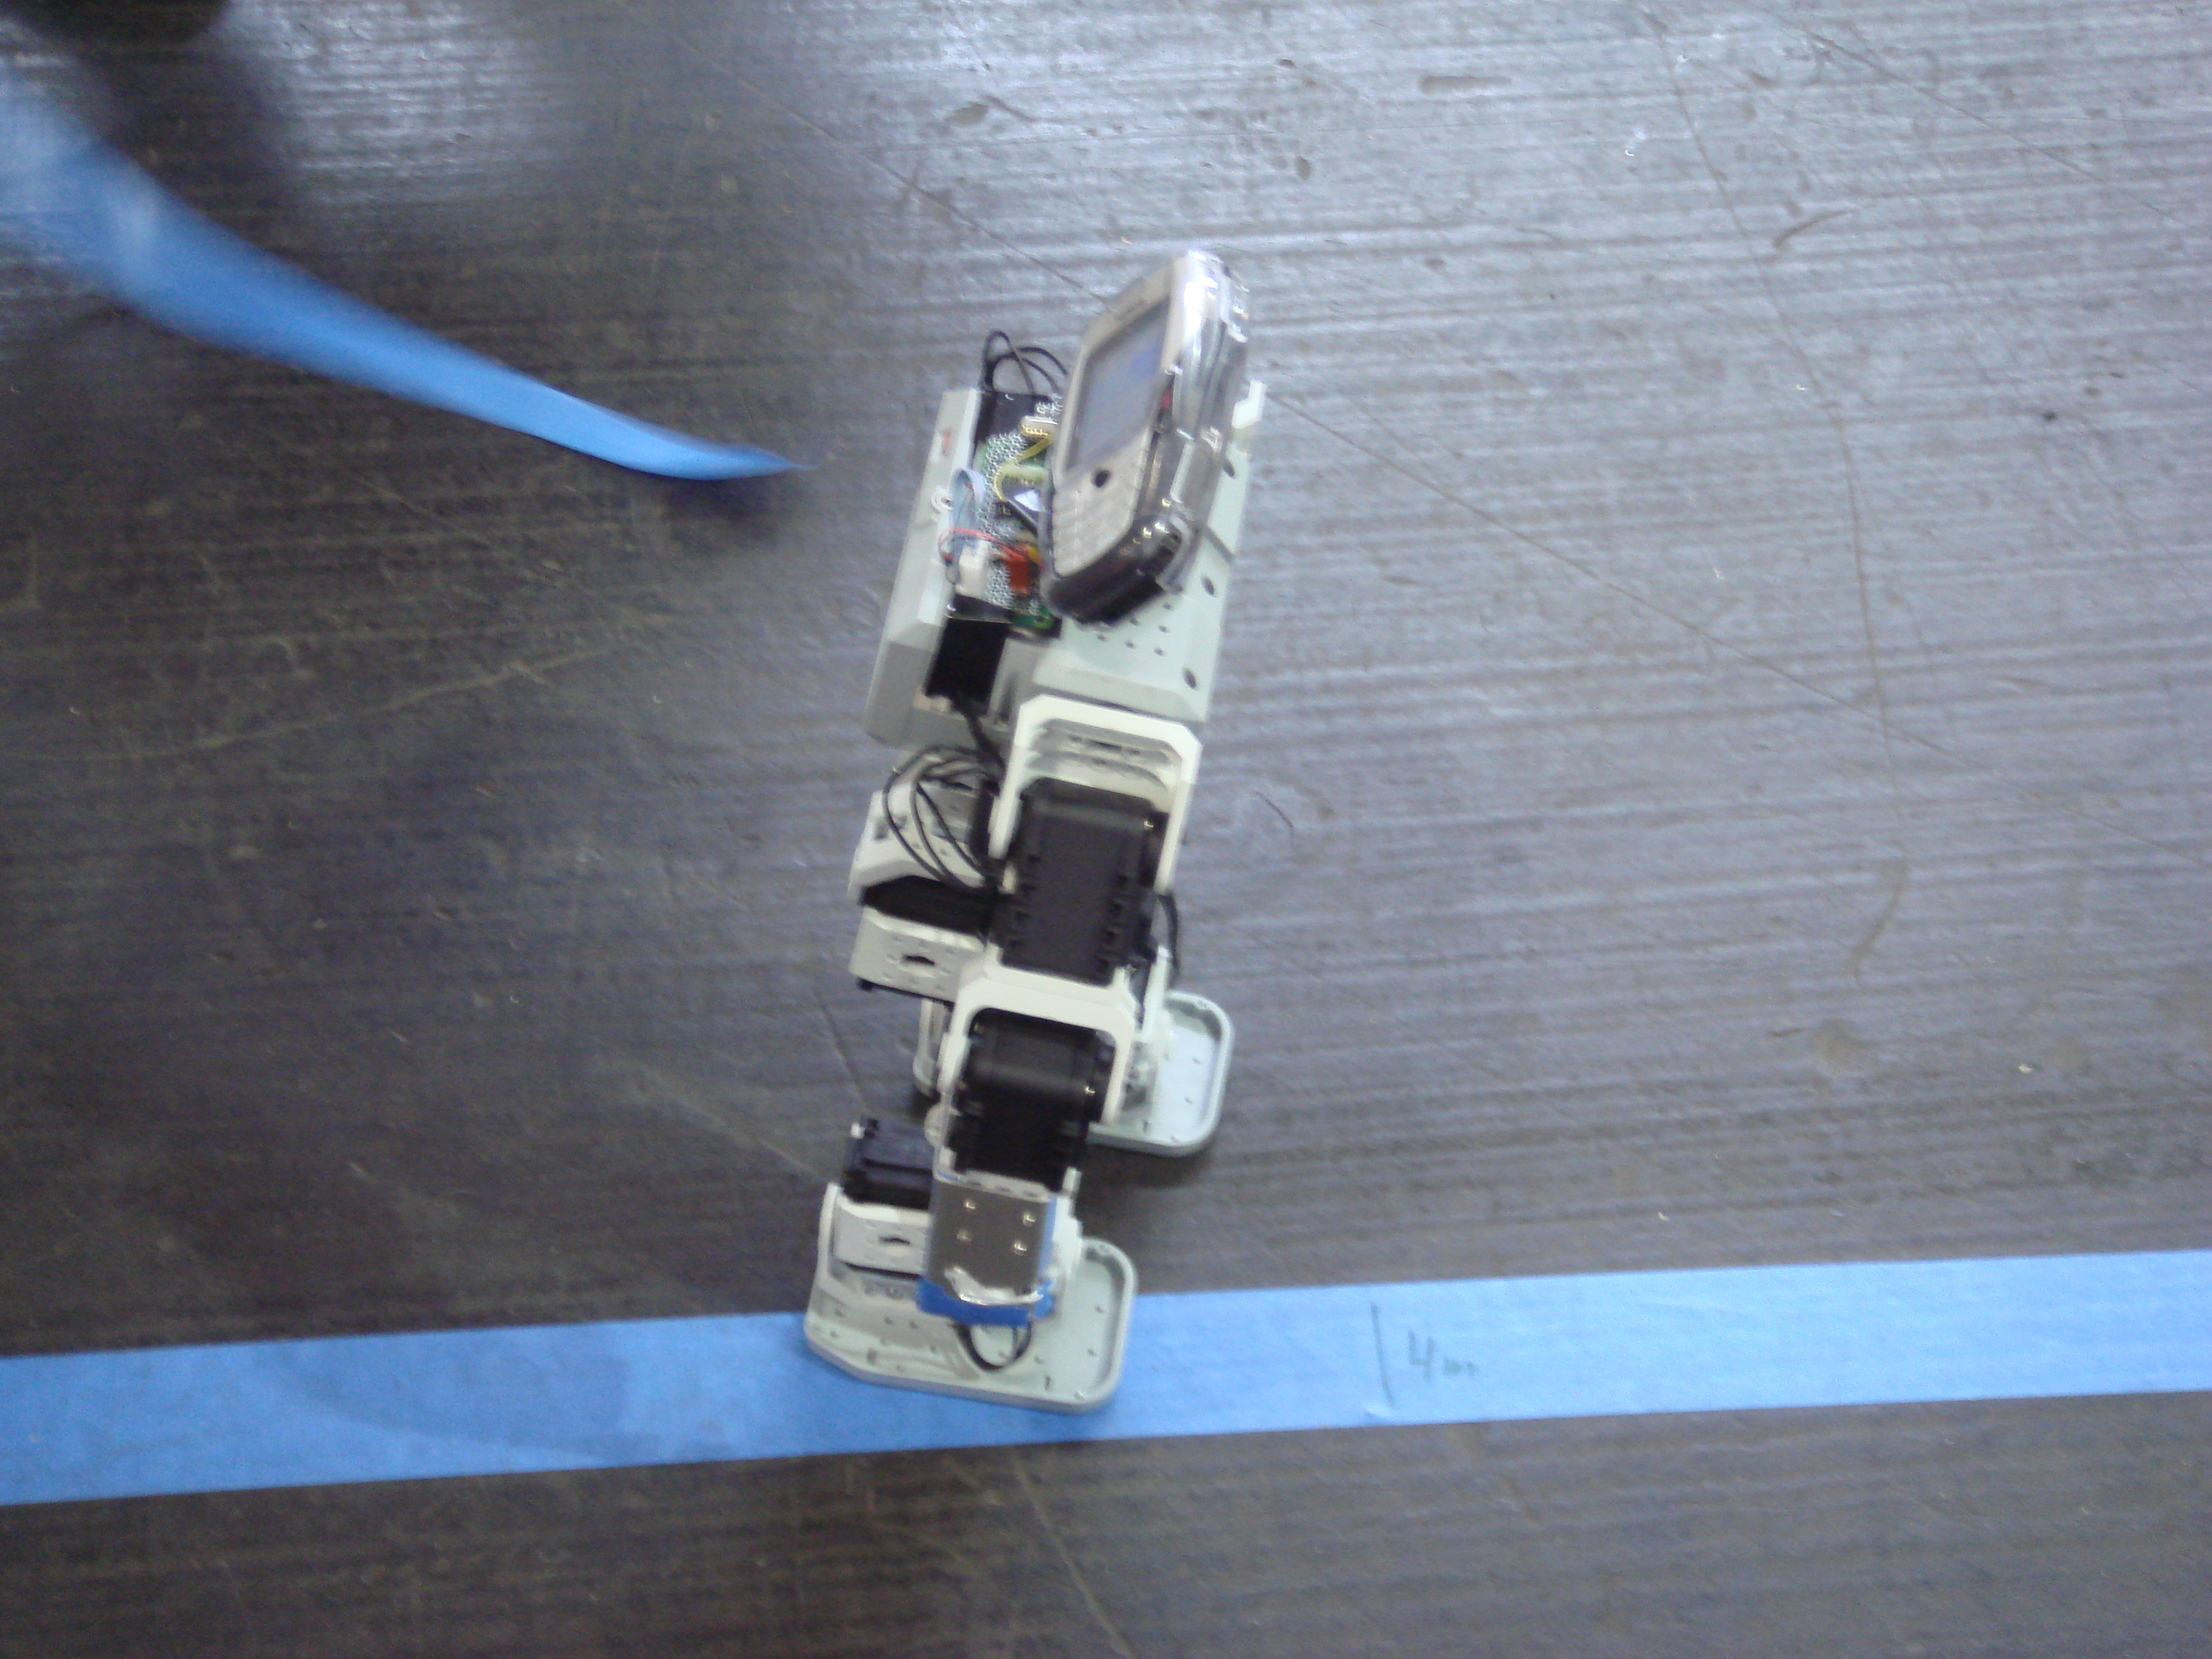
\includegraphics[width=0.7\textwidth]{Figures/marathon-track}
  \end{center}
  \caption{Marathon Track}
  \label{fig:marathon-track}
\end{figure}

\end{lawlist}

\law[MR]{Number of Robots}

\begin{lawlist}[MR]
\item A single robot competes in a match.
\end{lawlist}

\law[MR]{The Players}

Please refer to the general \HuroCup\ laws for a description of
the players.

\law[MR]{The Referee}

Please refer to the general \HuroCup\ laws for a description of
the referee.

\law[MR]{The Assistant Referee}

Please refer to the general \HuroCup\ laws for a description of
the assitant referee.

\law[MR]{Game Play}

\begin{lawlist}[MR]

\item Robots are assigned start numbers. The race commences with a
  staggered start of 3 minute intervals, that is the robot with start
  number $n$ will start 3 minutes after the robot with start number
  $n-1$.

\item The start of a run for a robot is signaled by the referee
  blowing the whistle. After the referee blows the whistle, the robot
  will walk towards the finish line.

\item \label{catch-up} A robot is faster than another robot, if its
  current movement speed along the path is higher than that of the
  other robot.

\item If the distance between the smaller and the faster robot is less
  than 50cm, then the referee will instruct the handler of the slower
  robot to remove his or her robot.

\item The referee will indicate to the handler of the slower robot
  from which position the slower robot is allowed to continue the
  race. The position for the slower robot to continue is approximately
  50cm behind the faster robot.

\item Each robot may have at most one human handler associated with
  it.

\item \label{handler1} The human handlers are not allowed to
  interfere in any way with other robots, the referee, or other human
  handlers.

\item \label{handler2} A human handler may only enter the playing
  field or touch his/her robot with the permission of the referee.

\item A robot has crossed the finish line when either
  foot of the robot crosses the finish plane and touches the ground in
  the area behind the finish line. The finish plane is the plane which
  intersects the playing field at a 90 degree angle at the back of the
  finish line.

\item The handler shall remove his/her assigned robot as soon as
  possible after it has crossed the finish line.

\item The end of the competition is signaled by the referee by blowing
  the whistle a second time. The referee terminates the competition
  if
  \begin{itemize}
    \item the maximum duration of the competition (1 hour) has
      elapsed.
  \item all robots have crossed the finish line,
  \item no more active robots remain in the competition.
  \end{itemize}

\end{lawlist}

\begin{decisions}
\item The minimum distance between two robots shall be at least 50cm
  at all times. 
\end{decisions}

\law[MR]{Fouls and Misconduct}

\begin{lawlist}[MR]

\item \label{inf-interference} Apart from~\ref{catch-up}, a robot is
  not allowed to interfere with another robot in any way. In case of
  multiple robots interfering with each other, the right of way goes
  to the faster robot.

\item A robot is not allowed to leave the track. A robot is considered
  to have left the track if the distance between the current position
  of the robot and the closest point on the centre line to that
  position is more than 50cm.

\item \label{inf-fix} The robot handler is not allowed to touch the
  robot. However, after being penalized for this infraction, the
  robot's handler may request permission from the referee to fix his
  robot. After having received permission from the referee, the helper
  may fix the robot. Please refer to~\ref{inf-batteries} for special
  laws regarding the batteries of the robot.

\item \label{inf-hurocup} Any infractions as listed by the general
  \HuroCup\ laws as far as they are applicable in this event.

\item Any team that commits one of the infractions listed
  in~\ref{inf-interference} to~\ref{inf-hurocup} will be penalized by
  a 2m push back by the referee. The robot must be placed 2m back
  towards the start line along the track. If the robot is less than 2m
  ahead of the start line, the robot shall be placed behind the start
  line. This is subject to laws~\ref{handler1} and~\ref{handler2}.

\item \label{inf-batteries} Not withstanding~\ref{inf-fix}, a team is
  not allowed to change the batteries during the competition, changing
  the batteries will immediately terminate the race for this robot.
\end{lawlist}

\law[MR]{Method of Scoring}

\begin{lawlist}[MR]
\item All robots that have not covered a maximum path distance of at least
  10m along the track are automatically awarded no rank and $0$
  points.
\item Among the robots that have covered more than 1m, the robots are
  ranked (i.e., 1st place, 2nd place) based on the maximum path distance.
\item All robots with the same maximum path distance are ranked based
  on the faster time to reach the maximum path distance.

\item The point allocation for robots is as follows:
  \begin{itemize}
  \item The first ranked robot is awarded $10$ points.
  \item The second ranked robot is awarded $8$ points.
  \item The third ranked robot is awarded $6$ points.
  \item The fourth, fifth, sixth, and seventh place robots are awarded
    $4$,$3$,$2$, and $1$ point respectively.  A summary of the point
    allocation for placings is shown in table~\ref{point-allocation}.

    \begin{table}
      \begin{center}
        \begin{tabular}{l|l}
          \hline
          Place & Points scored \\
          \hline
          1 (Winner) & 10 \\
          2          & 8 \\
          3          & 6 \\
          4          & 4 \\
          5          & 3 \\
          6          & 2 \\
          7          & 1 \\
          8, 9, ...  & 0 \\
          \hline
        \end{tabular}
      \end{center}
      \caption{Point allocation for placings in the \HuroCup\ events.}
      \label{point-allocation}
    \end{table}
  \end{itemize}

\item In case of a tie between $n$ robots with rank $k$, all robots
 will be awarded rank $k$ and receive the average of the scores for
 ranks $k$ to $k+n$.  For example, if the robots $A,B,C,D$ scored $10,
 8, 8, 4$ goals respectively, then robot $A$ will be declared the
 winner (1st place) and receive 10 points, both robots $B$ and $C$
 will be declared 2nd place finishers and receive $(8+6)/2=7$, and
 robot $D$ will be declared the fourth place finisher and receive $4$
 points.

\end{lawlist}

\section{Official World Records}
\label{sec:worldrecords}

This section contains the list of official world records for the
HuroCup Marathon competiton first introduced in the 2007 FIRA WorldCup
competiton.

\begin{center}
\begin{tabular}{|lllll|}
\hline
Date & Event & Team & Affiliation & Time \\
\hline
17th June 2007 & FIRA WorldCup 2007 & Hansaram & KAIST, Korea & 37:30:00 \\
\hline
\end{tabular}
\end{center}

\end{document}


% *** Local Variables: ***
% *** mode: LaTeX ***
% *** mode: outline-minor ***
% *** mode: auto-fill ***
% *** outline-regexp: "% !\\|\\\\\\(sub\\)*section" ***
% *** TeX-command-default: "LaTeX PDF" ***
% *** End: ***
